\setchapterpreamble[ur]{
  \dictum
  [Michèle Audin, \textit{Conseils aux auteurs de textes mathématiques}]
  {Un texte mathématique est, d’abord, un texte.}
  \vspace{1em}
}



\chapter{Writing text}

% According to \cite{mathoverflow_text} and Google~Translate the above quote may be translated as follows:
% \begin{center}
%   \enquote{A mathematical text is, before everything else, a text.}
% \end{center}
In this chapter we will talk about the more text focused aspects of writing mathematics with {\LaTeX}.
We will in particular talk about the interplay between the mathematical content and the text that surrounds it.




\section{Obey orthography}
\index{orthography}
\label{a mathematical text is a text}

A mathematical text has to obey the rules of the language that is it written in (e.g.~English, French, German or Russian).
A mathematical formula is part of the surrounding text, and has to be treated as such.





\section{Proper punctuation}



\subsection{A sentence ends with punctuation}
\index{punctuation!in formulas|(}

\Cref{a mathematical text is a text} has an important consequence:
If a sentence ends with a formula, then this formula need to be followed by some kind of punctuation (in most cases by a period).
The following example is very wrong:
\begin{showlatex}*{Very wrong punctuation in an equation}
It follows that
\[
  a^2 + b^2 = c^2
\]
.
This formula is important.
\end{showlatex}
The next example is also wrong:
\begin{showlatex}*{Wrong punctuation in an equation~I}
It follows that
\[
  a^2 + b^2 = c^2
\]
This formula is important.
\end{showlatex}
The following is still wrong:
\begin{showlatex}*{Wrong punctuation in an equation~II}
It follows that:
\[
  a^2 + b^2 = c^2
\]
This formula is important.
\end{showlatex}
The following example finally does it right:
\begin{showlatex}*{Right punctuation in an equation}
It follows that
\[
  a^2 + b^2 = c^2.
\]
This formula is important.
\end{showlatex}
But it is even better if we add some slight spacing between the formula and the period.
\begin{showlatex}*{Best punctuation in an equation}
It follows that
\[
  a^2 + b^2 = c^2 \,.
\]
This formula is important.
\end{showlatex}
This last approach is taken from \cite{tex_period}, which we strongly encourage the reader to check out.

\index{punctuation!in formulas|)}



\subsection{Punctuation in commutative diagrams?}
\index{punctuation!in commutative diagrams|(}
\index{commutative diagrams|(}

There is some disagreement in the mathematical community about whether a commutative diagram is allowed to include punctuation coming from the surrounding text.
The author is of the opinion that a commutative diagram should not contain any such punctuation.

There are two standard ways to achieve this:
One can finish up the sentence that precedes a commutative diagram beforehand:
\begin{showlatex}{Finishing the sentence before the commutative diagram}
  We consider the following commutative diagram:
  \[
    \begin{tikzcd}
        A
        \arrow{r}
        \arrow{d}
      &
        A'
        \arrow{d}
      \\
        C
        \arrow{r}
      &
        C'  
    \end{tikzcd}
  \]
  The horizontal arrows in this diagram are isomorphisms.
\end{showlatex}
But it often better to incorporate the diagram in the surrounding sentence in such a way that it contains no punctuation:
\begin{showlatex}{Incorporating the commutative diagram in the sentence}
  In the commutative diagram
    \[
    \begin{tikzcd}
        A
        \arrow{r}
        \arrow{d}
      &
        A'
        \arrow{d}
      \\
        C
        \arrow{r}
      &
        C'  
    \end{tikzcd}
  \]
  both horizontal arrows are isomorphisms.
\end{showlatex}

\index{punctuation!in commutative diagrams|)}
\index{commutative diagrams|)}



\subsection{Lists contain punctuation}
\index{punctuation!in lists|(}
\index{lists}

Text that is organized using list environments still obeys the rules of punctuation.
Consider the following counterexample:
\begin{showlatex}{Wrong punctuation in lists}
  A set $B$ is a basis of $V$ if
  \begin{enumerate}
    \item
      $B$ is linearly independent
    \item
      $B$ is a generating set
  \end{enumerate}
\end{showlatex}
To figure out the correct punctuation simply remove the surrounding list and consider the resulting text.
In the above example this gives the following:
\begin{center}
  A set $B$ is a basis of $V$ if $B$ is linearly independent $B$ is a generating set
\end{center}
This is not a proper sentence, and should instead be as follows:
\begin{center}
  A set $B$ is a basis of $V$ if $B$ is linearly independent and $B$ is a generating set.
\end{center}
The above counterexample should hence read as follows:
\begin{showlatex}{Right punctuation in lists~I}
  A set $B$ is a basis of $V$ if
  \begin{enumerate}
    \item
      $B$ is linearly independent and
    \item
      $B$ is a generating set.
  \end{enumerate}
\end{showlatex}
There are also some other acceptable versions:
\begin{showlatex}{Right punctuation in lists~II}
  A set $B$ is a basis of $V$ if it satisfies the following two conditions:
  \begin{enumerate}
    \item
      $B$ is linearly independent.
    \item
      $B$ is a generating set.
  \end{enumerate}
\end{showlatex}

\index{punctuation!in lists|)}



\subsection{Hyphen and dashes}

\subsubsection{Know your lines}

In {\LaTeX} there are (at least) four line-like symbols which need to be distinguished, the hyphen\massindex[punctuation]{hyphen}, the en~dash\massindex[punctuation]{en~dash}, the em~dash\massindex[punctuation]{em~dash} and the minus~sign\index{minus sign}.
See \cref{dash list} for their {\LaTeX}~code and look.
\begin{table}[tb]
  \begin{center}
  \begin{tabular}{@{}lll@{}}
    \toprule
    \theading{name}
    &
    \theading{code}
    &
    \theading{output}
    \\
    \midrule
    hyphen
    &
    \inlinecode{-}
    &
    -
    \\
    en~dash
    &
    \inlinecode{--}
    &
    --
    \\
    em~dash
    &
    \inlinecode{---}
    &
    ---
    \\
    minus~sign
    &
    \inlinecode{\$-\$}
    &
    $-$
    \\
    \bottomrule
  \end{tabular}
  \end{center}
  \caption{Kinds of hyphen and dashes.}
  \label{dash list}
\end{table}
Each of these symbols plays its own role, and these roles depend both on language and on convention.
For mathematical writing in English the following usages are important:
\begin{myitemize}
  \item
    For \enquote{$n$-dimensional} and \enquote{$3$-manifold}, use the hyphen.
  \item
    For combining names as in \enquote{Cauchy--Schwarz inequality} use the en~dash.
  \item
    To interrupt a sentence{---}as done here{---}use the em~dash without surrounding space, or -- if you’re feeling British -- use the en~dash surrounded by space.
\end{myitemize}
For more information about the use of hyphen and dashes in the English language we refer to \cite[6.75--6.94]{chicago}.

To underline how language dependent the usage of hyphen and dashes is we’re considering in \cref{cgc names} how the the Clebsch--Gordan are called in different languages, as taken from Wikipedia.
(We use the same font%
\footnote{Namely~\enquote{Noto~Serif~CJK~JP}.}
for all examples to allow a better comparison.)
\begin{table}[tb]
  \begin{center}
  \begin{tabular}{@{}lll@{}}
    \toprule
    \theading{language}
    &
    \theading{name}
    &
    \theading{dash used}
    \\
    \midrule
    English
    &
    \multilang{Clebsch–Gordan coefficients}
    &
    en~dash
    \\
    German
    &
    \multilang{Clebsch-Gordan-Koeffizienten}
    &
    hyphen
    \\                                                      
    French
    &
    \multilang{coefficients de Clebsch-Gordan}
    &
    hyphen
    \\
    Dutch
    &
    \multilang{Clebsch-Gordan-coëfficienten}
    &
    hyphen
    \\
    Russian
    &
    \multilang{Коэффициенты Клебша — Гордана}
    &
    em~dash
    \\
    Japanese
    &
    \multilang{クレブシュ–ゴルダン係数}
    &
    en~dash
    \\
    \bottomrule
  \end{tabular}
  \end{center}
  \caption{The Clebsch--Gordan coefficients in different languages.}
  \label{cgc names}
\end{table}

\subsubsection{Don’t put a hyphen in math~mode}

A non-trivial amount of people makes the mistake of putting a hyphen\massindex[punctuation]{hyphen} into math~mode.
\begin{showlatex}{An accidental hyphen in math~mode}
Let~$A$ be an $R-$module.
\end{showlatex}
We can see that we don’t get a hyphen but a minus sign.
We hence need to place the symbol~\inlinecode{-} outside of the math environment.
\begin{showlatex}{Proper placement of the hyphen}
Let~$A$ be an $R$-module.
\end{showlatex}



\subsection{Correct spacing after a period}
\label{spacing after dots}
\index{spacing!after a period|(}

\subsubsection{The problem}

Not all periods are treated equally by {\LaTeX}:
If a period is both followed by whitespace and not preceded by an uppercase letter then {\LaTeX} will assume that this period is supposed to end a sentence.
It will some introduce some additional space following this period.
The effect of this can be seen in \cref{period spacing}.
\begin{table}
  \begin{center}
  \begin{tabular}{@{}r@{\hskip 2.7em}r@{\hskip 2.7em}l@{\hskip 2.7em}l@{}}
    \toprule
    \multicolumn{2}{c}{\theading{right aligned}}
    &
    \multicolumn{2}{c}{\theading{left aligned}}
    \\
    \cmidrule(r{2.7em}){1-2}\cmidrule{3-4}
    \scalebox{3.5}[3.5]{x. x}
    &
    \scalebox{3.5}[3.5]{x. X}
    &
    \scalebox{3.5}[3.5]{x. x}
    &
    \scalebox{3.5}[3.5]{X. x}
    \\
    \scalebox{3.5}[3.5]{X. x}
    &
    \scalebox{3.5}[3.5]{X. X}
    &
    \scalebox{3.5}[3.5]{x. X}
    &
    \scalebox{3.5}[3.5]{X. X}
    \\
    \bottomrule
  \end{tabular}
  \end{center}
  \caption{Spacings after a period (with a zoom of factor~$3.5$).}
  \label{period spacing}
\end{table}

We can see from the first two columns of~\cref{period spacing} (by considering the positions of the periods) that the spacing in~\enquote{\inlinecode{x.~*}} is larger then the corresponding spacing in~\enquote{\inlinecode{X.~*}}.
This happens because {\LaTeX} thinks that the period in~\enquote{\inlinecode{x. *}} is supposed to end a sentence.
We can also see from the first two tables that this difference of spacing occurs both if the following letter is lower case and if it is upper case.
We can see from the third and fourth column that the amount of additional spacing does not depenend on whether the following letter is in lower case or upper case.

\subsubsection{First Solution}

The default behaviour of {\LaTeX}, to put additional space after a period that ends a sentence, is outdated.
So it is best to just deactivate it.
This can via the command \comname{frenchspacing}\massindex[spacing!after a period]{frenchspacing}[\comname].
By putting this command in the preamble, the whole document will be affected.

\begin{showcode}{Using \comname{frenchspacing}}
  \documentclass[a4paper, 10pt]{scrartcl}

  \frenchspacing

  \begin{document}

  No additional space after a sentence in this document.

  \end{document}
\end{showcode}

The additional spacing can also be reenabled by \comname{nofrenchspacing}\massindex[spacing!after a period]{nofrenchspacing}[\comname].

\begin{showlatex}{Using \comname{nofrenchspacing}}
  \frenchspacing
  Observe the spacing. Between the preceeding period.
  \nonfrenchspacing\\
  Observe the spacing. Between the preceeding period.
\end{showlatex}

\subsubsection{Second Solution}

If the default behavior should be kept, then one needs to do more manual work.

We can use the command~\enquote{\comname{ }} -- which we will write for readability as~\comname{(space)}\massindex[spacing!after a period]{(space)}[\comname] -- to tell~{\LaTeX} that a preceding period is not meant to end a sentence.
We can similarly use the command~\comname{@}\massindex[spacing!after a period]{"@}[\comname] to tell {\LaTeX} that the following period is ending a sentence.
Consider the following example:
\begin{showlatex}{Proper spacing after periods}
Imagine now some old and long-dead English kings, e.g.\ Henry III and Henry IV\@.
(Kings not named Henry are also okay.)
\end{showlatex}
Note that in the above example one should also use ties~\inlinecode{\customtexttilde} (as explained in \cref{non-breakable space}) to ensure that the Henries don’t lose their number.
\begin{showlatex}{Proper spacing after periods, and using~\inlinecode{\customtexttilde}}
Imagine now some old and long-dead English kings, e.g.\ Henry~III and Henry~IV\@.
(Kings not named Henry are also okay.)
\end{showlatex}

It should be pointed out that if a problematic period is followed by a closing parenthesis, a closing bracket, or quotations marks then then the problematic spacing will still occur after these symbols.
Lets consider the following example (where we use the otherwise forbidden~\comname{\tbs} to compare the versions).
\begin{showlatex}{Spacings after periods followed by parentheses or quotation marks}
Many colours (e.g. red, blue, etc.) are supported by \enquote{ColorX}. Even purple! \\
Many colours (e.g.\ red, blue, etc.) are supported by \enquote{ColorX}. Even purple! \\
Many colours (e.g.\ red, blue, etc.)\ are supported by \enquote{ColorX}. Even purple! \\
Many colours (e.g.\ red, blue, etc.)\ are supported by \enquote{ColorX}\@. Even purple!
\end{showlatex}

The problem of a sentence ending with an upper case letter does not occur if this letter is in math~mode.
\begin{showlatex}{Upper case mathematics followed by a period}
Let $f$ be an endomorphism of $X$.
Then $f$ is an isomorphism or $f = 0$.\\
Let $f$ be an endomorphism of $X$\@.
Then $f$ is an isomorphism or $f = 0$.\\
Let $f$ be an endomorphism of $X$.\ 
Then $f$ is an isomorphism or $f = 0$.
\\
Let $f$ be an endomorphism of $\operatorname{X}$.
Then $f$ is an isomorphism or $f = 0$.\\
Let $f$ be an endomorphism of $\operatorname{X}$\@.
Then $f$ is an isomorphism or $f = 0$.\\
Let $f$ be an endomorphism of $\operatorname{X}$.\ 
Then $f$ is an isomorphism or $f = 0$.
\end{showlatex}

In view of the upcoming \cref{non-breakable space} we get a problem:
What if we want the space after an abbreviation, as in~\enquote{i.e.~word}, not to be broken?
Should we then write~\inlinecode{i.e.{\tbs} word} or~\inlinecode{i.e.{\customtexttilde}word}?

In this case we write~\inlinecode{i.e.{\customtexttilde}word}, since the tie~\inlinecode{\customtexttilde} already contains the effect of~\comname{(space)}.
Consider for this the following example:
\begin{showlatex}{Spacing of~\inlinecode{\customtexttilde} and~\enquote{\inlinecode{{\tbs} }}}
Let $M$ be a $2$-manifold, e.g. $M = S^2$. \\
Let $M$ be a $2$-manifold, e.g.\ $M = S^2$. \\
Let $M$ be a $2$-manifold, e.g.~$M = S^2$.
\end{showlatex}

To summarize this \lcnamecref{spacing after dots}:
If an abbreviation or some non-word things appear one should pay heed to periods which may occur at their ends.
Most of these special cases are covered by paying attention to~\enquote{i.e.~*} and~\enquote{e.g.~*}.

We refer to \cite[19.5.1, 19.6]{latex2e_manual} for more information on this topic.

\index{spacing!after a period|)}





\section{Text layout}



\subsection{Use non-breakable space}
\label{non-breakable space}

If two expressions in text mode are separated by a space or a hyphen then {\LaTeX} may separate these expressions in the output \filename{pdf}-file by a line break\index{line breaks!in text mode}.
But such line breaks are often undesirable and can sometimes be downright wrong.
Comsider for this the following examples:
\begin{myitemize}
  \item
    Abbreviations like~\enquote{Prof.~Dr.~John Doe}.
  \item
    Cmbinations of words and numbers like~\enquote{Lemma~5}.
  \item
    Combinations of mathematics and words like~\enquote{$3${\nbd}dimensional}.
\end{myitemize}
In such cases one needs to prevent the line break.

\subsubsection{Line breaks at a space}

No line break will occur if the tie\index{\customtexttilde}\index{tie}\index{unbreakable!space} symbol~\inlinecode{\customtexttilde} is used instead of a space.
Consider for this the following example:
% fragile example
\begin{showlatex}*{An unwanted line break at a space}
Text text text text text text text text text text text text text, so by Lemma 35 text text text text text text text text
\end{showlatex}
We don’t want a line break to occur in the term~\enquote{Lemma~35} and thus introduce a tie.
\begin{showlatex}*{Using~\inlinecode{\customtexttilde} to prevent unwanted line breaks at spaces}
Text text text text text text text text text text text text text, so by Lemma~35 text text text text text text text text
\end{showlatex}

\subsubsection{Line breaks at a hyphen}

Consider the following example:
% % fragile example
\begin{showlatex}{An unwanted line break at a hyphen}
  textextext textextext textextext textextext textextext textextext textext 123456-dimensional textextext
\end{showlatex}
To prevent a line break at the hyphen\massindex[punctuation]{hyphen} we put~\comname{nobreakdash} before it:
\begin{showlatex}{Using~\comname{nobreakdash} to prevent unwanted line breaks at hyphens}
  textextext textextext textextext textextext textextext textextext textext 123456\nobreakdash-dimensional textextext
\end{showlatex}
The command~\comname{nobreakdash} works not only with hyphens but also with en~dashes\index{unbreakable!dash}\massindex[punctuation]{en~dash} and em~dashes\index{unbreakable!dash}\massindex[punctuation]{em~dash}.



\subsection{Don’t use \comtitle{\tbs} or \comtitle{newline}}

The proper way to separate two succeeding paragraphs\index{paragraphs}\index{indentation!of paragraphs} in {\LaTeX} is to leave an empty line between them.
\begin{showlatex}*{New paragraphs done right}
This is the first paragraph.
It consists of multiples lines to make this example better.

This is a second paragraph.
It also consists of multiple lines to make this example even more better.

This one is the third and last paragraph in this example.
It also consists of multiple lines.
\end{showlatex}
Note that new paragraphs start indented.

The use of~\comname{\tbs}\massindex{\tbs}[\comname] or~\comname{newline}\massindex{newline}[\comname] doesn’t actually end a paragraph but only forces a line break.\index{line breaks!in text mode}
\begin{showlatex}*{New \enquote{paragraphs} done wrong}
This is the first paragraph in a counterexample.\\
This is not a new paragraph.
The text is just forced to start a new line.\newline
This one is also not a new paragraph.
But this whole thing looks ugly.
\end{showlatex}
The use of \comname{\tbs} and \comname{newline} is only for starting new rows in matrices, tables and arrays.%
\footnote{
  In this text we sometimes use~\comname{\tbs} to tweak examples, to make certain lines more comparable.
  This is done purely for technical purposes and should not be done for actual mathematical writings.
}
Don’t use is to separate paragraphs.



\subsection{Text consisting of lists}

The two list~environments~\envname{enumerate} and~\envname{itemize} contain by default certain indentations, that can be problematic in mathematical writing.

\subsubsection{Identation compared to the left~margin}

There is by default some indentation between the left~margin of the text area and the item labels.
This is meant to visually separate the list from the surrounding text.
But in mathematical writing there often occur lists that don’t have a surrounding text.
The most prominent example for this are propositions (and their proofs) that consist of multiple statements:
\begin{showlatex}{A list without surrounding text}
\begin{theorem}
  Let $G$ be a finite group.
  \begin{enumerate}
    \item
      If $H$ is subgroup of $G$ then $\operatorname{ord}(H)$ divides $\operatorname{ord}(G)$.
    \item
      If $g$ is any element of $G$ then $\operatorname{ord}(g)$ divides $\operatorname{ord}(G)$.
    \item
      Every group of prime order is cyclic.
    \item
      If $p$ is a prime divisor of $\operatorname{ord}(G)$ then $G$ contains an element of order $p$.
  \end{enumerate}
\end{theorem}
\end{showlatex}

In such cases one should remove the identation between the left~margin of the text area and the item~labels, as explained in \cref{list indentation with enumitem}.
\begin{showlatex}{A list without surrounding text}
\begin{theorem}
  Let $G$ be a finite group.
  \begin{enumerate}[wide = 0pt, leftmargin=*]
    \item
      If $H$ is subgroup of $G$ then $\operatorname{ord}(H)$ divides $\operatorname{ord}(G)$.
    \item
      If $g$ is any element of $G$ then $\operatorname{ord}(g)$ divides $\operatorname{ord}(G)$.
    \item
      Every group of prime order is cyclic.
    \item
      If $p$ is a prime divisor of $\operatorname{ord}(G)$ then $G$ contains an element of order $p$.
  \end{enumerate}
\end{theorem}
\end{showlatex}



\subsubsection{Theorems and proofs beginning with a list}

If a theorem-like~environment\index{theorem-like environments} or a the environment~\envname{proof}\massindex[\piname{amsthm}]{proof}[\envname] begins with a list~environment then the first item of this list will not be aligned with the other list items:
\begin{showlatex}{Improper aligned of list items}
\begin{lemma}
\begin{enumerate}
  \item
    Every group $G$ is isomorphic to its opposite group $G^{\mathrm{op}}$.
  \item
    A group $G$ equals its opposite group $G^{\mathrm{op}}$ if and only if it is abelian.
\end{enumerate}
\end{lemma}
\end{showlatex}

One way to circumvent this problem is by inserting the command~\comname{leavevmode}\massindex{leavevmode}[\comname] before the beginning of the list.
\begin{showlatex}{Proper aligned of list items with~\comname{leavevmode}}
\begin{lemma}
\leavevmode
\begin{enumerate}
  \item
    Every group $G$ is isomorphic to its opposite group $G^{\mathrm{op}}$.
  \item
    A group $G$ equals its opposite group $G^{\mathrm{op}}$ if and only if it is abelian.
\end{enumerate}
\end{lemma}
\end{showlatex}
The problem with this approach is that it allows a line break to occur at the position of~\comname{leavevmode}.
So it may happen that the header of the theorem-like environment of proof environment occurs at the very bottom of the page while the list appears only on the next page.
(This looks quite horrible.)

As far as the author is aware there exists no good solution for this problem.%
\footnote{The package~\packname{ntheorem}\massindex[packages]{ntheorem}[\packname] is allegedly able to address this problem, at the price of introducing new problems.}
A good way of coping with this problem is to circumvent it by introducing some text before the list~environment:
\begin{showlatex}{Proper aligned of list items by introducing text}
\begin{lemma}
Let $G$ be a group with opposite group $G^{\mathrm{op}}$. 
\begin{enumerate}
  \item
    The groups $G$ and $G^{\mathrm{op}}$ are isomorphic.
  \item
    The groups $G$ and $G^{\mathrm{op}}$ are equal if and only if $G$ is abelian.
\end{enumerate}
\end{lemma}
\end{showlatex}
An seen above we should also eliminate the indentation between the left~margin of the text~area and the item~labels:
\begin{showlatex}{Proper aligned of list items by introducing text}
\begin{lemma}
Let $G$ be a group with opposite group $G^{\mathrm{op}}$. 
\begin{enumerate}[wide = 0pt, leftmargin=*]
  \item
    The groups $G$ and $G^{\mathrm{op}}$ are isomorphic.
  \item
    The groups $G$ and $G^{\mathrm{op}}$ are equal if and only if $G$ is abelian.
\end{enumerate}
\end{lemma}
\end{showlatex}



\section{Mathematics in text}



\subsection{Don’t break inline mathematics}
\label{breaking inline math}

When inline formulas or inline equations are too long or badly placed then it can happen that a line break\index{line breaks!in text mode} occurs inside the formula, tearing it apart:
% fragile example
\begin{showlatex}[before lower = {\binoppenalty=100}, after lower = {\binoppenalty = \maxdimen}]{Line break in inline math}
The most important formula of all times is without a doubt is my mind $1 + 2 + 3 + 4 = 10$.
Truly a work of genius!
% fragile example
\end{showlatex}
This horrible affront to nature can thankfully be eliminated by setting the penalties~\comname{binoppenalty}\massindex[penalties]{binoppenality}[\comname] and~\comname{relpenalty}\massindex[penalties]{relpenalty}[\comname] to their maximum value, which can be accessed via the command~\comname{maxdimen}\massindex{maxdimen}[\comname].
\begin{showlatex}{Preventing inline math in inline math}
% in the preamble:
\binoppenalty = \maxdimen
\relpenalty   = \maxdimen
% in the main text:
The most important formula of all times is without a doubt is my mind $1 + 2 + 3 + 4 = 10$.
Truly a work of genius!
\end{showlatex}



\subsection{Don’t begin a sentence with a mathematical symbol}

Don’t begin a sentence with a mathematical symbol.
Consider the following example:
\begin{showlatex}{Mathematics at the beginning of a sentence}
\begin{theorem}
  $\mathbf{Mod}(R)$ is an abelian category.
\end{theorem}
\end{showlatex}
Instead do the following:
\begin{showlatex}{No mathematics at the beginning of a sentence}
\begin{theorem}
  The category $\mathbf{Mod}(R)$ is abelian.
\end{theorem}
\end{showlatex}

An exception to the above rule are lists\index{lists}, in which short entries may start with a math symbol.
Consider for this the following example.
\begin{showlatex}{List items beginning with mathematics}
Let $V$ be a finite dimensional vector space.
Let $U$ and $W$ be two linear subspaces of $V$ of complementary dimensions, i.e.\ such that $\dim V = \dim U + \dim W$.
Then the following conditions are equivalent:
\begin{enumerate}[label = \roman*)]
  \item
    $V = U \oplus W$.
  \item
    $V = U + W$.
  \item
    $U \cap W = 0$.
\end{enumerate}
\end{showlatex}



\subsection{Don’t put two formulas next to each other}

One should not put two mathematical formulas right next to each other.
Consider the following example:
\begin{showlatex}{Not properly separating mathematics}
Then $f^2 = g$,$f$ is differentiable and $f = \exp(h)$.
\end{showlatex}
The human eye (and brain) parses this sentence as follows:
\begin{center}
  Then
  \quad
  $f^2 = g$,$f$
  \quad
  is differentiable and
  \quad
  $f = \exp(h)$.
\end{center}
But this betrays the actual content of the sentence.
This problem can be fixed by introducing some more text.
One solution is the following:
\begin{showlatex}{Properly separating mathematics~I}
Then $f^2 = g$, the function $f$ is differentiable and $f = \exp(h)$.
\end{showlatex}
This sentence is parsed as follows:
\begin{center}
  Then
  \quad
  $f^2 = g$,
  \quad
  the function
  \quad
  $f$
  \quad
  is differentiable and
  \quad
  $f = \exp(h)$.
\end{center}
The following is another solution:
\begin{showlatex}{Properly separating mathematics~II}
The function $f$ satisfies $f^2 = g$, it is differentiable and $f = \exp(h)$.
\end{showlatex}
This sentence is parsed as follows:
\begin{center}
  The function
  \quad
  $f$
  \quad
  satisfies
  \quad
  $f^2 = g$,
  \quad
  it is differentiable and
  \quad
  $f = \exp(h)$.
\end{center}



\subsection{Don’t begin a line with a mathematical symbol (optional)}

One interesting idea for inline mathematics is to never start a line with a mathematical symbol.
This can be achieved by prefixing every inline mathematical formula by a tie~\inlinecode{\customtexttilde}.
The author has taken this approach from~\cite{nomath_at_line}.





\section{Text in mathematics}


\subsection{Use \comtitle{text}}

When text needs to be used in math~mode the command~\comname{text} is to be used.
\begin{showcode}{Syntax of \comname{text}}
\text{normal text in math mode}
\end{showcode}
Let’s start with the following horrible example:
\begin{showlatex}{Missing text in math~mode}
Let $A \coloneqq \{ x \in [0,1] : x \; is \; rational \}$.
\end{showlatex}
This next one looks a bit better, but is still not okay:
\begin{showlatex}[label = {wrong math mode position}]{Wrong way of using text in math~mode}
Let $A \coloneqq \{ x \in [0,1] : x \text{ is rational} \}$.
\end{showlatex}
Instead do this:
\begin{showlatex}[label = {right math mode position}]{Right way of using text in math~mode}
Let $A \coloneqq \{ x \in [0,1] : \text{$x$ is rational} \}$.
\end{showlatex}
Note that the right code reflects the actual structure\index{structure of an expression} of the displayed expression:
Indeed, the diagram in \cref{structure tree of definition} shows the structure of the given expression.
\begin{figure}[tb]
  \begin{center}
    % the following diagram uses the "trees" library
    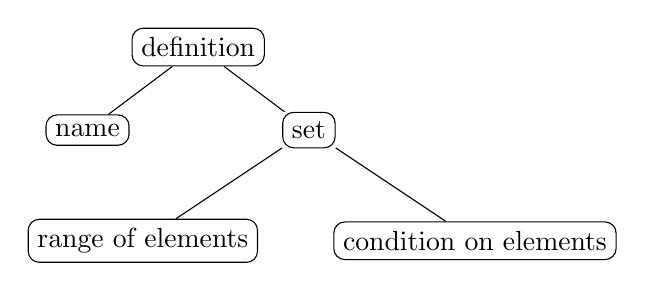
\begin{tikzpicture}[
      every node/.style = {shape=rectangle, rounded corners, draw, align=center, level distance = 5em},
      level 1/.style = {sibling distance = 8em, level distance = 3em},
      level 2/.style = {sibling distance = 12em, level distance = 4em}
      ]
      \node {definition}
        child { node {name} }
        child { node {set} 
                child { node {range of elements} }
                child { node {condition on elements} }
              }
        ;
    \end{tikzpicture}
  \end{center}
  \caption{Structure tree of the definition.}
  \label{structure tree of definition}
\end{figure}
To get the right kind of code we assign to each node of this diagram the desired content, and whether this node is mathematics or text.
If a node contains both mathematics and text then it is primary a text, which just happens to contain some mathematics.
We arrive at the diagram in \cref{structure tree of math}.
\begin{figure}[tb]
  \begin{center}
    % the following diagram uses the "trees" library
    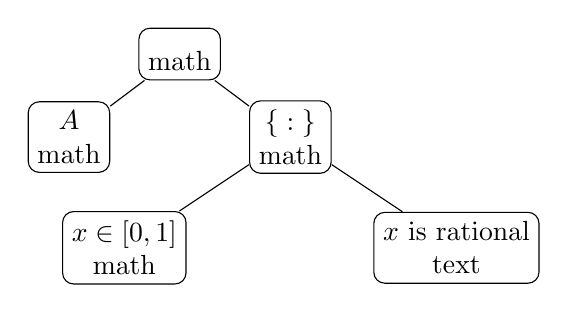
\begin{tikzpicture}[
      every node/.style = {shape=rectangle, rounded corners, draw, align=center, level distance = 5em},
      level 1/.style = {sibling distance = 8em, level distance = 3em},
      level 2/.style = {sibling distance = 12em, level distance = 4em}
      ]
      \node {$\coloneqq$ \\ math}
        child { node {$A$ \\ math} }
        child { node {$\{ \; : \; \}$ \\ math} 
                child { node {$x \in [0,1]$ \\ math} }
                child { node {$x$ is rational \\ text} }
              }
        ;
    \end{tikzpicture}
  \end{center}
  \caption{Structure tree of the mathematical expression.}
  \label{structure tree of math}
\end{figure}
By transforming this diagram node-wise into code we arrive at \cref{right math mode position}.
Note that both the nodes~\enquote{$x \in [0,1]$} and~\enquote{$x$ is rational} both contain mathematics, but that the second is actually a text.
It is therefore not proper to combine these two math~modes, as done in \cref{wrong math mode position}.



\subsection{Put space around text in display mathematics}

Sometimes a single line of displayed mathematics end with some text, as in the following example.
\begin{showlatex}{Wrong spacing around text in math~mode~I}
Therefore
\[
  g h g^{-1}
  =
  h
  \text{for all $g, h \in G$}.
\]
\end{showlatex}
In such a case one needs to put space\index{spacing!in math~mode} between the mathematics and the text.
This space should not be part of the text.
Consider the following counterexample:
\begin{showlatex}{Wrong spacing around text in math~mode~II}
Therefore
\[
  g h g^{-1}
  =
  h
  \text{ for all $g, h \in G$.}
\]
\end{showlatex}
Instead the spacing should be put between the formula and the text.

In the above example, where a single block of mathematics is follows by a single block of text which contains quantifiers for the previous formula, one should use the spacing~\comname{qquad}\massindex[spacing]{qquad}[\comname]:
\begin{showlatex}{Right spacing around text in math~mode~I}
Therefore
\[
  g h g^{-1}
  =
  h
  \qquad
  \text{for all $g, h \in G$.}
\]
\end{showlatex}
Sometimes two blocks of mathematics are separated by a short text.
In this case one should use the spacing~\comname{quad}\massindex[spacing]{quad}[\comname] on both sides of the text:
\begin{showlatex}{Right spacing around text in math~mode~II}
That $gh = hg$ can equivalently be expressed as
\[
  g h g^{-1} = h
  \quad\text{and}\quad
  h g h^{-1} = g \,.
\]
\end{showlatex}
It may even be appropriate to use~\comname{qquad} on both sides when more space is needed.



\subsection{Use \comtitle{intertext} and \comtitle{shortintertext}}

Multi-line display mode environments like \envname{gather*}\massindex[display math environment, multi-line mathematics]{gather*}[\envname] and \envname{align*}\massindex[display math environment, multi-line mathematics]{align*}[\envname] (see \cref{display environments}) can be interrupted by inserting some text via the commands~\comname{intersect}\massindex[text in math~mode]{intertext}[\comname] and~\comname{shortintertext}\massindex[text in math~mode]{shortintertext}[\comname] to insert some text between different lines of mathematics.
This is particularly useful to combine multiple \envname{align*}~environments into a single one, which then allows for a common alignment\index{aligning formulas} of all lines.

The following is an example for what we don’t want.
\begin{showlatex}{Two non-aligned blocks}
We consider the equalities
\begin{align*}
  H
  &= a_1 + a_2 + a_3 + a_4 \\
  &= b_1 + b_2 + b_3 + b_4 + b_5 + b_6 \\
  &= c_1 + c_2 + c_3 + c_4 + c_5
\end{align*}
and
\begin{align*}
  I
  &= d_1 + d_2 + d_3 + d_4 + d_5 + d_6 \\
  &= e_1 + e_2 + e_3 \\
  &= f_1 + f_2 + f_3 + f_4 + f_5 \,.
\end{align*}
\end{showlatex}
Note the annoying misalignment of the equality signs of the two \envname{align*}~environments.
We can solve this problem by using only one \envname{align*}~environment and inserting the text~\enquote{and} by using the command~\comname{intertext}:
\begin{showlatex}{Two aligned blocks}
We consider now the equalities
\begin{align*}
  H
  &= a_1 + a_2 + a_3 + a_4 \\
  &= b_1 + b_2 + b_3 + b_4 + b_5 + b_6 \\
  &= c_1 + c_2 + c_3 + c_4 + c_5
\intertext{and}
  I
  &= d_1 + d_2 + d_3 + d_4 + d_5 + d_6 \\
  &= e_1 + e_2 + e_3 \\
  &= f_1 + f_2 + f_3 + f_4 + f_5 \,.
\end{align*}
\end{showlatex}

The command~\comname{shortintertext} works in the same way as~\comname{intertext} but inserts less vertical space\index{spacing} around it.
To see the effects of~\comname{shortintertext} let us start with the following example:
\begin{showlatex}*{Two non-aligned equalities}
It follows from the identity
\[
  a = b
\]
that
\[
  b = a \,,
\]
which proves the theorem.
\end{showlatex}
We naturally want to align the two equality signs, which we by using a single \comname{align*}~environment together with~\comname{intertext}, as explained above:
\begin{showlatex}*{Two aligned equalities with too much space}
It follows from the identity
\begin{align*}
  a &= b
\intertext{that}
  b &= a \,,
\end{align*}
which proves the theorem.
\end{showlatex}
But we can see that the inserted~\comname{intersect} puts a large distance between the two formulas.
This distance is far too large for our taste.
We can solve this problem by using~\comname{shortintertext} instead of~\comname{intertext}, as the following example shows:
\begin{showlatex}*{Two aligned equalities with proper space}
It follows from the identity
\begin{align*}
  a &= b
\shortintertext{that}
  b &= a \,,
\end{align*}
which proves the theorem.
\end{showlatex}





\section{Mathematics as text}



\subsection{Don’t abuse math as text}

Again similar to \cref{no logical symbols} one should not abuse mathematical symbols as words:

A mathematical symbol can often replace parts of a sentence, in particular a verb.
\begin{showlatex}{Right way of using mathematical symbols as words}
Then $a = b$ and thus $b \leq c$.
\end{showlatex}
But this use of mathematics should be treated with care, and not abused:
\begin{showlatex}{Wrong way of using mathematical symbols as words}
The integer $a$ is $< 0$ and thus $\notin \mathbb{N}$.
\end{showlatex}
This kind of tortue is highly illegal, so don’t do it!


\subsection{Logical symbols don’t replace text}
\label{no logical symbols}

Mathematicians often abuse logical symbols\index{logical symbols} like
\[
  \exists \,,
  \quad
  \forall \,,
  \quad
  \implies \,,
  \quad
  \iff
\]
as replacements for written out words.
This is okay in handwriting and on blackboards, but it is not okay in a properly written out mathematical text.
\begin{showlatex}{Abuse of quantifiers}
It follows that $\forall y \in B$ that $\exists x \in A$ with $f(x) = y$.
\end{showlatex}
One needs to instead write out the used quantifiers.
\begin{showlatex}{Writing out quantifiers}
It follows that for every element $y \in B$ there exists an element $x \in A$ with $f(x) = y$.
\end{showlatex}
In this example one should also write out the element relation:
\begin{showlatex}{Best use of quantifiers}
It follows that for every element $y$ of $B$ there exists an element $x$ of $A$ with $f(x) = y$.
\end{showlatex}

The use of the above logical symbols is of course okay if they are used in their actual logical function:
\begin{showlatex}{Okay way to use logical symbols}
  Let $f \colon X \to Y$ be a morphism in a category $\mathcal{C}$.
  Then
  \begin{align*}
    {}&
      \text{$f$ is an epimorphism}
    \\
    \iff{}&
    \bigl[
    \forall Z \in \operatorname{Ob}(\mathcal{C}):
    \forall g, h \in \mathcal{C}(Y,Z):
    g \circ f = h \circ f \implies g = h
    \bigr]
    \\
    \iff{}&
    \bigl[
    \forall Z \in \operatorname{Ob}(\mathcal{C}):
    \text{$f^* \colon \mathcal{C}(Y,Z) \to \mathcal{C}(X,Z)$ is injective}
    \bigr]
    \\
    \implies{}&
    \text{$f^* \colon \mathcal{C}(Y,-) \to \mathcal{C}(X,-)$ is a monomorphism in~$\mathbf{Fun}(\mathcal{C}, \mathbf{Set})$}
  \end{align*}
\end{showlatex}



\subsection{Don’t use \enquote{iff}}
\index{iff}
\label{no iff}

Similarly to \cref{no logical symbols} abbreviations like~\enquote{iff} need to be written out in a proper mathematical text.




